% !TEX TS-program = lualatex
% !BIB TS-program = biber
%\documentclass[handout]{beamer}
\documentclass{beamer}
\newcommand{\misoclasstinytitleslide}{Partially based on material by:  Rob Fergus, Nikhil Srivastava,\\[-1em] 
Yiannis Koutis, Joshua Batson, Daniel Spielman}
%{Partially based on material by:  Branislav Kveton,  \\[-1em]  Partha Niyogi, Rob Fergus}
\newcommand{\misoclassdate}{}
\input{../common/misomva}
\usepackage{verbatim}
\usepackage{listings}
\usepackage[customcolors]{hf-tikz}
\usepackage{color}
\usepackage{cancel}
%\usepackage[defaultmono]{droidmono}
\newcommand{\nbskip}{\vspace{-\baselineskip}}
%\newcommand{\hbskip}{\vspace{.5\baselineskip}}
\newcommand{\nhbskip}{\vspace{-.5\baselineskip}}

\definecolor{mygreen}{rgb}{0,0.6,0}
\definecolor{mygray}{rgb}{0.5,0.5,0.5}
\definecolor{mymauve}{rgb}{0.58,0,0.82}

\definecolor{Code}{rgb}{0,0,0}
\definecolor{Decorators}{rgb}{0.5,0.5,0.5}
\definecolor{Numbers}{rgb}{0.5,0,0}
\definecolor{MatchingBrackets}{rgb}{0.25,0.5,0.5}
\definecolor{Keywords}{rgb}{0,0,1}
\definecolor{self}{rgb}{0,0,0}
\definecolor{Strings}{rgb}{0,0.63,0}
\definecolor{Comments}{rgb}{0,0.63,1}
\definecolor{Backquotes}{rgb}{0,0,0}
\definecolor{Classname}{rgb}{0,0,0}
\definecolor{FunctionName}{rgb}{0,0,0}
\definecolor{Operators}{rgb}{0,0,0}
\definecolor{Background}{rgb}{0.98,0.98,0.98}

\lstset{ %
backgroundcolor=\color{white},   % choose the background color; you must add \usepackage{color} or \usepackage{xcolor}
basicstyle=\fdmfamily\footnotesize,        % the size of the fonts that are used for the code
breakatwhitespace=false,         % sets if automatic breaks should only happen at whitespace
breaklines=true,                 % sets automatic line breaking
captionpos=b,                    % sets the caption-position to bottom
commentstyle=\color{mygreen},    % comment style
deletekeywords={\dots},            % if you want to delete keywords from the given language
escapeinside={\%*}{*)},          % if you want to add LaTeX within your code
extendedchars=true,              % lets you use non-ASCII characters; for 8-bits encodings only, does not work with UTF-8
frame=single,	                   % adds a frame around the code
keepspaces=true,                 % keeps spaces in text, useful for keeping indentation of code (possibly needs columns=flexible)
language=Python,                 % the language of the code
% Comments
commentstyle=\color{Comments}\slshape,
% Strings
stringstyle=\color{Strings},
morecomment=[s][\color{Strings}]{"""}{"""},
morecomment=[s][\color{Strings}]{'''}{'''},
% keywords
morekeywords={import,from,class,def,for,while,if,is,in,elif,else,not,and,or,print,break,continue,return,True,False,None,access,as,,del,except,exec,finally,global,import,lambda,pass,print,raise,try,assert},
keywordstyle={\color{Keywords}\bfseries},
% additional keywords
morekeywords={[2]@invariant},
keywordstyle={[2]\color{Decorators}\slshape},
emph={self},
emphstyle={\color{self}\slshape},
otherkeywords={*,\dots},            % if you want to add more keywords to the set
numbers=left,                    % where to put the line-numbers; possible values are (none, left, right)
numbersep=5pt,                   % how far the line-numbers are from the code
numberstyle=\tiny\color{mygray}, % the style that is used for the line-numbers
rulecolor=\color{black},         % if not set, the frame-color may be changed on line-breaks within not-black text (e.g. comments (green here))
showspaces=false,                % show spaces everywhere adding particular underscores; it overrides 'showstringspaces'
showstringspaces=false,          % underline spaces within strings only
showtabs=false,                  % show tabs within strings adding particular underscores
stepnumber=1,                    % the step between two line-numbers. If it's 1, each line will be numbered
tabsize=2,	                   % sets default tabsize to 2 spaces
title=\lstname                   % show the filename of files included with \lstinputlisting; also try caption instead of title
}


\newcommand{\consindent}[1]{
    \begin{itemize}
        \item[{
\includegraphics[height=0.7\baselineskip]{../img/arrow_list}}] #1
    \end{itemize}
}


%%% part daniele
\usepackage{etex}
\TPshowboxesfalse
\textblockorigin{0mm}{0mm}

\definecolor{rouge1}{RGB}{226,0,38}  % red P
\definecolor{orange1}{RGB}{243,154,38}  % orange P
\definecolor{jaune}{RGB}{254,205,27}  % jaune P
\definecolor{blanc}{RGB}{255,255,255} % blanc P

\definecolor{rouge2}{RGB}{230,68,57}  % red S
\definecolor{orange2}{RGB}{236,117,40}  % orange S
\definecolor{taupe}{RGB}{134,113,127} % taupe S
\definecolor{gris}{RGB}{91,94,111} % gris S
\definecolor{bleu1}{RGB}{38,109,131} % bleu S
\definecolor{bleu2}{RGB}{28,50,114} % bleu S
\definecolor{vert1}{RGB}{133,146,66} % vert S
\definecolor{vert3}{RGB}{20,200,66} % vert S
\definecolor{vert2}{RGB}{157,193,7} % vert S
\definecolor{darkyellow}{RGB}{233,165,0}  % orange S
\definecolor{lightgray}{rgb}{0.9,0.9,0.9}
\definecolor{darkgray}{rgb}{0.6,0.6,0.6}

\setbeamertemplate{navigation symbols}{}
\setbeamertemplate{blocks}[rounded]
\setbeamercolor{block title}{bg=bleu2,fg=white}%bg=background, fg= foreground
\setbeamercolor{block body}{bg=lightgray}%bg=background, fg= foreground

\renewcommand{\sfdefault}{lmss}
\sffamily

%\newcommand{\ycol}[1]{\textcolor{darkyellow}{\textit{#1}}}

\newcommand{\rcolb}[1]{\textcolor{red}{\textit{\textbf{#1}}}}
\newcommand{\gcolb}[1]{\textcolor{vert3}{\textit{\textbf{#1}}}}
\newcommand{\bcolb}[1]{\textcolor{blue}{\textit{\textbf{#1}}}}
\newcommand{\ycolb}[1]{\textcolor{darkyellow}{\textit{\textbf{#1}}}}

\newcommand{\eqrcol}[1]{\textcolor{red}{#1}}
\newcommand{\eqgcol}[1]{\textcolor{vert3}{#1}}
\newcommand{\eqbcol}[1]{\textcolor{blue}{#1}}
\newcommand{\eqrcolb}[1]{\textcolor{red!70}{\mathbf{#1}}}
\newcommand{\eqgcolb}[1]{\textcolor{vert3!70}{\mathbf{#1}}}
\newcommand{\eqbcolb}[1]{\textcolor{blue!70}{\mathbf{#1}}}
\newcommand{\eqycol}[1]{\textcolor{darkyellow}{#1}}

%\newcommand{\otoprule}{\midrule[\heavyrulewidth]}

\colorlet{redp}{red!20} % vert S
\colorlet{greenp}{vert3!20} % vert S
\colorlet{bluep}{blue!20} % vert S

\usepackage{adjustbox}

% Highlight and cancel commands are defined in misomva.tex

\newcommand{\bookboxx}[1]{
\par\medskip\noindent
\framebox[\columnwidth]{
\begin{minipage}{0.98\columnwidth} {\par\smallskip#1\par\smallskip} \end{minipage} } \par\medskip }

\setbeamersize{text margin left=1cm,text margin right=1cm}
\tikzstyle{every picture}+=[remember picture]

\newcommand{\incarrow}{{
\includegraphics[height=0.7\baselineskip]{../img/arrow_list}}}
\newcommand{\consarrow}{{\hspace*{.1pt} 
\includegraphics[height=0.7\baselineskip]{../img/arrow_list}}\;}

% Change margins for slides
\newenvironment{changemargin}[2]{% 
  \begin{list}{}{% 
    \setlength{\topsep}{0pt}% 
    \setlength{\leftmargin}{#1}% 
    \setlength{\rightmargin}{#2}% 
    \setlength{\listparindent}{\parindent}% 
    \setlength{\itemindent}{\parindent}% 
    \setlength{\parsep}{\parskip}% 
  }% 
  \item[]}{\end{list}} 


%\include{mathdef}  % File not available in slides folder
\newcommand{\ie}{i.e.\xspace}
\newcommand{\eg}{e.g.\xspace}

\newcommand{\greycite}[1]{{\small \textcolor{gray}{\cite{#1}}}}
%%%

\begin{document}
% Topic-specific title slide
\newcommand{\topictitle}{Large-Scale Machine Learning on Graphs}
\newcommand{\topicsubtitle}{Computational Bottlenecks and Challenges}
\renewcommand{\misoclasstinytitleslide}{Partially based on material by:  Rob Fergus, Nikhil Srivastava,\\[-1em] Yiannis Koutis, Joshua Batson, Daniel Spielman}

\MakeTopicSlide

\begin{frame}
\frametitle{Large scale Machine Learning on Graphs}
\begin{tabular}{>{\centering\arraybackslash}m{0.5\textwidth} >{\centering\arraybackslash}m{0.5\textwidth}}
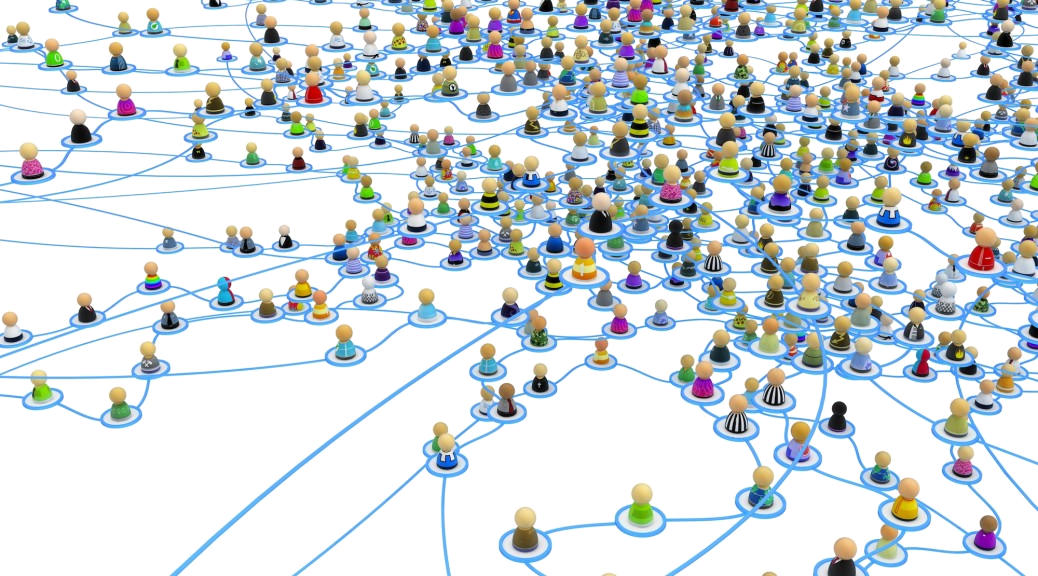
\includegraphics[width=0.45\textwidth]{../img/facebook} & 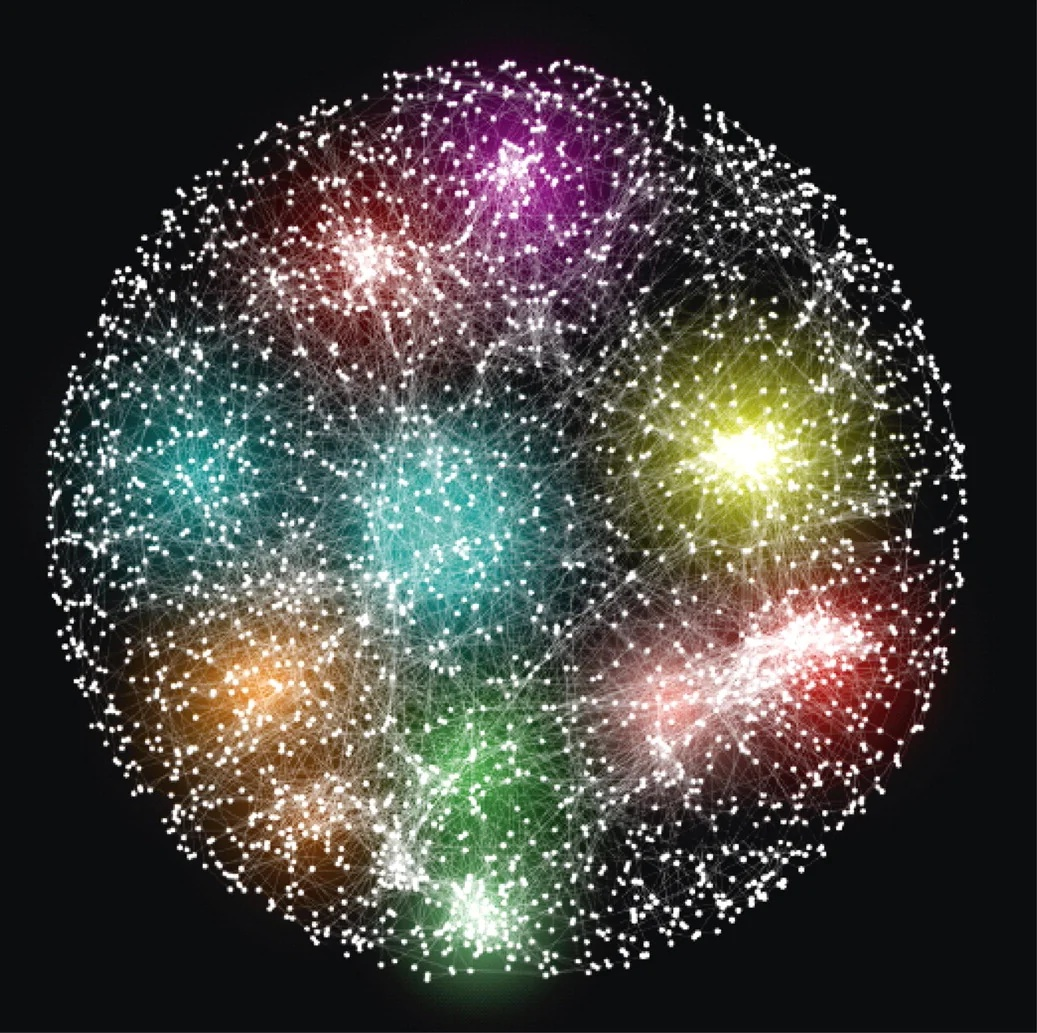
\includegraphics[width=0.45\textwidth]{../img/yeast}\\
\vspace{1cm} {\tiny \url{http://blog.carsten-eickhoff.com}} & \vspace{1cm}{\tiny Botstein et al.}
\end{tabular}
\end{frame}
%%%%%%%%%%%%%%%%%%%%%%%%%%%%%%%%%%%%%%%%%%%%%%%%%%%%%%%%%%%%%
\begin{frame}
\frametitle{Are we large yet?}
\begin{center}
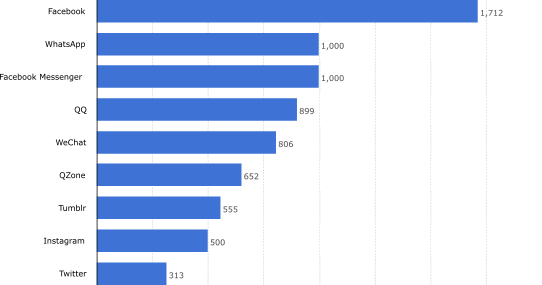
\includegraphics[width=\textwidth]{../img/users}\\*
"One \textbf{trillion} edges: graph processing at Facebook-scale."\\*
Ching et al., VLDB 2015
\end{center}
\end{frame}
%%%%%%%%%%%%%%%%%%%%%%%%%%%%%%%%%%%%%%%%%%%%%%%%%%%%%%%%%%%%%
\begin{frame}
\frametitle{Computational bottlenecks}
\begin{center}
In theory:
\begin{tabular}{>{\centering\arraybackslash}m{0.45\textwidth} >{\centering\arraybackslash}m{0.45\textwidth}}
\textbf{Space} & \textbf{Time} \\
$[\cO(m),\cO(n^2)]$ to store
&$\cO(n^2)$ to construct \newline
$\cO(n^3)$ to run algorithms\\
\end{tabular}
\vspace{1.5\baselineskip}

\pause
In practice:
 \begin{itemize}
 \item 2012 Common Crawl Corpus:
 \begin{itemize}
    \item[] 3.5 Billion pages (45 GB)
    \item[] 128 Billion edges (331 GB)
 \end{itemize}
 \pause
 \item Pagerank on Facebook Graph:
    \begin{itemize}
    \item[] 3 minutes per iteration, hundreds of iterations, tens of hours
    on 200 machines, run once per day
    \end{itemize}
\end{itemize}
\end{center}
\end{frame}
%%%%%%%%%%%%%%%%%%%%%%%%%%%%%%%%%%%%%%%%%%%%%%%%%%%%%%%%%%%%%
\begin{frame}
\frametitle{Two phases}
\begin{itemize}[<+-| alert@+>]\addtolength{\itemsep}{0.75\baselineskip}
\item[1]  Preprocessing:
\begin{itemize}
\item[] \textbf{From vectorial data:} Collect a dataset $\bX \in \mathbb{R}^{n \times d}$,
  construct a graph $\bG$ using a similarity function
\item[] \textbf{Prepare the graph:} Need to check if graph is connected, make it directed/undirected, build Laplacian
\item[] \textbf{Load it on the machine:} On a single machine if possible, if not find smart way to distribute it
\end{itemize}
\item[2] Run your algorithm on the graph
\end{itemize}
\end{frame}
%%%%%%%%%%%%%%%%%%%%%%%%%%%%%%%%%%%%%%%%%%%%%%%%%%%%%%%%%%%%%

\begin{frame}
\frametitle{Large scale graph construction}

\textbf{Time} bottleneck
\begin{itemize}[<+-| alert@+>]\addtolength{\itemsep}{0.25\baselineskip}
\item Constructing $k$-nn graph takes $\bO(n^2\log(n))$, too slow
\item Constructing $\varepsilon$ graph takes $\bO(n^2)$, still too slow
\item In both cases bottleneck is the same, given a node finding close nodes ($k$ neighbours or $\varepsilon$ neighbourhood)
\end{itemize}
\pause
\vspace{\baselineskip}
\yellbox{Fundamental limit: just looking at all similarities already too slow.}

\pause
\vspace{\baselineskip}
\questionbox{Can we find close neighbours without checking all distances?}
\end{frame}

\begin{frame}
\frametitle{Large scale graph construction}

\yellbox{Split your data in small subset of close points}

\vspace{0.5\baselineskip}
Can find efficiently some (not all) of the neighbours.
\pause
\begin{itemize}[<+-| alert@+>]\addtolength{\itemsep}{0.25\baselineskip}
\item Iterative Quantization
\item KD-Trees -- Cover Trees -- NN search is $\cO(\log \nodes)$ per node
\item Locality Sensitive Hashing (LSH)
\end{itemize}

\pause

More general problem: \questionbox{learning good codeword representation}

\end{frame}

\begin{frame}
\frametitle{Storing graph in memory}

Main bottleneck: \textbf{space}.

As a Fermi (back-of-the-envelope) problem
\begin{itemize}[<+->]
\item Storing a graph with $m$ edges require to store $m$ tuples $(i,j,w_{i,j})$ of 64 bit ($8$ bytes) doubles or int.
\item The largest compute-optimized cloud instances have 64+ cores, but only 128 GB of memory.
\item We can store $128*1024^3/(3*8) \sim 5.7 \times 10^9$ (5.7 billion) edges in a single machine
memory.
\end{itemize}
\end{frame}

\begin{frame}
\frametitle{Storing graph in memory}

But wait a minute
\begin{itemize}[<+->]\addtolength{\itemsep}{0.75\baselineskip}
    \item Natural graphs are sparse.
    \consindent{
    For some it is true, for some it is false (e.g. Facebook average user has 300 friends, Twitter averages 208 followers)
    \questionbox{Subcomponents are very dense, and they grow denser over time}}
    \item I will construct my graph sparse
    \consindent{\questionbox{Losing large scale relationship, losing regularization}}
    \item I will split my graph across multiple machines
    \consindent{Your algorithm does not know that.
    \item[] \questionbox{What if it needs nonlocal data? Iterative algorithms?}
    \item[] More on this later}
\end{itemize}
\end{frame}


\MakeLastSlide
\end{document}
